\chapter{Outputs and Reports}\label{app:outputs}

This appendix reproduces the reports and outputs produced by the system on the final corpus, exactly as generated (model text is typeset from its Markdown; nothing has been edited for correctness).

\section{Analysis Report: GATE CS (2011--2026)}
Papers: 26; years: 2011--2026; questions: 1691; questions per paper by type: MCQ 36.5, NAT 23.4, MSQ 5.2; questions depending on a figure: 9.6\%.
\begin{center}\small\begin{tabular}{@{}lccc@{}}\toprule \textbf{Unit / subject} & \textbf{Marks/paper} & \textbf{Share (\%)} & \textbf{Trend}\\\midrule
General Aptitude & 14.85 & 14.8 & stable\\
Algorithms & 10.27 & 10.2 & stable\\
Programming and Data Structures & 9.77 & 9.7 & stable\\
Discrete Mathematics & 8.31 & 8.3 & stable\\
Operating System & 7.69 & 7.7 & stable\\
Theory of Computation & 7.46 & 7.4 & stable\\
Computer Networks & 7.42 & 7.4 & stable\\
Computer Organization and Architecture & 7.0 & 7.0 & stable\\
Databases & 7.0 & 7.0 & stable\\
Digital Logic & 6.12 & 6.1 & stable\\
Compiler Design & 5.35 & 5.3 & stable\\
Probability and Statistics & 3.96 & 3.9 & stable\\
Linear Algebra & 3.0 & 3.0 & stable\\
Calculus & 2.35 & 2.3 & stable\\
\bottomrule\end{tabular}\end{center}
\noindent\textbf{Top 15 topics by hot score}\par\smallskip
{\small\begin{longtable}{@{}p{6.4cm}p{3.6cm}ccc@{}}\toprule \textbf{Topic} & \textbf{Unit} & \textbf{Hot} & \textbf{Marks/paper} & \textbf{Years}\\\midrule\endhead
Verbal Aptitude: grammar, vocabulary, reading comprehension, analogies & General Aptitude & 100.0 & 7.42 & 16/16\\
Programming in C and recursion & Programming and Data Structures & 81.1 & 4.69 & 16/16\\
Quantitative Aptitude: arithmetic, percentages, ratios, data interpretation, mensuration & General Aptitude & 67.9 & 4.35 & 15/16\\
Memory hierarchy: cache, main memory and secondary storage & Computer Organization and Architecture & 62.1 & 3.0 & 15/16\\
Graph traversals, minimum spanning trees and shortest paths & Algorithms & 60.7 & 2.77 & 16/16\\
Memory management and virtual memory: paging, page replacement & Operating System & 57.2 & 2.46 & 16/16\\
Trees, binary search trees and binary heaps & Programming and Data Structures & 56.9 & 2.73 & 16/16\\
Spatial Aptitude: shapes, rotation, mirror images, paper folding, patterns & General Aptitude & 53.5 & 1.88 & 11/16\\
Regular expressions and finite automata & Theory of Computation & 49.2 & 2.58 & 16/16\\
Relational model: relational algebra, tuple calculus, SQL & Databases & 47.9 & 2.92 & 16/16\\
Context-free grammars and push-down automata & Theory of Computation & 43.7 & 1.85 & 11/16\\
Boolean algebra and minimization & Digital Logic & 41.5 & 2.04 & 14/16\\
Graphs: connectivity, matching, colouring & Discrete Mathematics & 40.8 & 2.12 & 15/16\\
IP addressing: IPv4, CIDR, subnetting, fragmentation, ARP, DHCP, ICMP, NAT & Computer Networks & 40.3 & 1.92 & 14/16\\
Parsing: LL, LR, SLR, LALR & Compiler Design & 39.0 & 2.31 & 15/16\\
\bottomrule\end{longtable}}
\noindent\textbf{Bloom's taxonomy distribution:} Understand 43.7\%, Apply 29.1\%, Analyze 15.7\%, Remember 9.9\%, Create 1.4\%, Evaluate 0.2\%.\par
\smallskip\noindent\textbf{Recurring concepts:}\begin{itemize}[leftmargin=1.4em,itemsep=1pt]
\item (0.86) GATE 2014 CS3 Q43 / GATE 2017 CS1 Q24: CPU and I/O scheduling
\item (0.81) GATE 2014 CS3 Q43 / GATE 2019 CS Q51: CPU and I/O scheduling
\item (0.81) GATE 2017 CS1 Q24 / GATE 2019 CS Q51: CPU and I/O scheduling
\item (0.73) GATE 2016 CS2 Q57 / GATE 2017 CS1 Q24: CPU and I/O scheduling
\item (0.72) GATE 2014 CS2 Q63 / GATE 2024 CS2 Q59: Graph traversals, minimum spanning trees and shortest paths
\item (0.71) GATE 2016 CS2 Q57 / GATE 2019 CS Q51: CPU and I/O scheduling
\end{itemize}

\section{Analysis Report: GATE DA (2024--2026)}
Papers: 4; years: 2024--2026; questions: 250; questions per paper by type: MCQ 37.2, MSQ 11.0, NAT 14.2; questions depending on a figure: 10.0\%.
\begin{center}\small\begin{tabular}{@{}lccc@{}}\toprule \textbf{Unit / subject} & \textbf{Marks/paper} & \textbf{Share (\%)} & \textbf{Trend}\\\midrule
Probability and Statistics & 18.5 & 19.2 & rising\\
Programming, Data Structures and Algorithms & 14.75 & 15.3 & falling\\
Machine Learning & 14.25 & 14.8 & stable\\
Database Management and Warehousing & 12.0 & 12.5 & rising\\
General Aptitude & 10.25 & 10.6 & rising\\
Linear Algebra & 10.25 & 10.6 & falling\\
Artificial Intelligence & 8.75 & 9.1 & falling\\
Calculus and Optimization & 7.5 & 7.8 & falling\\
\bottomrule\end{tabular}\end{center}
\noindent\textbf{Top 12 topics by hot score}\par\smallskip
{\small\begin{longtable}{@{}p{6.4cm}p{3.6cm}ccc@{}}\toprule \textbf{Topic} & \textbf{Unit} & \textbf{Hot} & \textbf{Marks/paper} & \textbf{Years}\\\midrule\endhead
File organization and indexing & Database Management and Warehousing & 100.0 & 5.5 & 3/3\\
Discrete and continuous random variables: Bernoulli, binomial, Poisson, uniform, exponential, normal & Probability and Statistics & 94.1 & 6.5 & 3/3\\
Verbal Aptitude: grammar, vocabulary, reading comprehension, analogies & General Aptitude & 86.5 & 4.5 & 3/3\\
Mean, variance, covariance, correlation, conditional expectation & Probability and Statistics & 79.8 & 4.75 & 3/3\\
Classification: logistic regression, k-nearest neighbour, naive Bayes, linear discriminant analysis, support vector machine, decision trees & Machine Learning & 72.9 & 5.75 & 3/3\\
Programming in Python & Programming, Data Structures and Algorithms & 70.5 & 4.75 & 3/3\\
Functions of a single variable: limits, continuity, differentiability & Calculus and Optimization & 61.5 & 4.25 & 3/3\\
Counting, axioms of probability, conditional probability, Bayes theorem, independence & Probability and Statistics & 60.8 & 4.75 & 3/3\\
Matrices, rank, determinant, inverse, projection, orthogonal and idempotent matrices & Linear Algebra & 54.6 & 3.5 & 3/3\\
Quantitative Aptitude: arithmetic, percentages, ratios, data interpretation, mensuration & General Aptitude & 52.3 & 3.25 & 3/3\\
Search: informed, uninformed and adversarial search & Artificial Intelligence & 51.8 & 4.25 & 3/3\\
Logic: propositional and predicate logic & Artificial Intelligence & 49.9 & 3.0 & 3/3\\
\bottomrule\end{longtable}}
\noindent\textbf{Bloom's taxonomy distribution:} Apply 38.8\%, Understand 27.2\%, Analyze 21.6\%, Remember 10.0\%, Evaluate 1.2\%, Create 1.2\%.\par
\smallskip\noindent\textbf{Recurring concepts:}\begin{itemize}[leftmargin=1.4em,itemsep=1pt]
\item (0.66) GATE 2024 DA (sample) Q53 / GATE 2026 DA Q56: Neural networks: multi-layer perceptron, feed-forward networks
\end{itemize}

\section{Analysis Report: Mathematics-II (university, 2025)}
Papers: 1; years: 2025--2025; questions: 30; questions per paper by type: DESCRIPTIVE 30.0; questions depending on a figure: 0.0\%.
\begin{center}\small\begin{tabular}{@{}lccc@{}}\toprule \textbf{Unit / subject} & \textbf{Marks/paper} & \textbf{Share (\%)} & \textbf{Trend}\\\midrule
Higher Order Linear Differential Equations & 40.0 & 25.6 & stable\\
Residue Calculus and Complex Series & 36.0 & 23.1 & stable\\
Vector Calculus and Theorems & 30.0 & 19.2 & stable\\
Complex Analysis and Mapping & 26.0 & 16.7 & stable\\
First Order Ordinary Differential Equations & 24.0 & 15.4 & stable\\
\bottomrule\end{tabular}\end{center}
\noindent\textbf{Top 10 topics by hot score}\par\smallskip
{\small\begin{longtable}{@{}p{6.4cm}p{3.6cm}ccc@{}}\toprule \textbf{Topic} & \textbf{Unit} & \textbf{Hot} & \textbf{Marks/paper} & \textbf{Years}\\\midrule\endhead
Residue Theorem and Contour Integration & Residue Calculus and Complex Series & 100.0 & 26.0 & 1/1\\
Power Series Solutions and Legendre Polynomials & Higher Order Linear Differential Equations & 76.9 & 20.0 & 1/1\\
Analytic Functions and Cauchy-Riemann Equations & Complex Analysis and Mapping & 61.5 & 16.0 & 1/1\\
First Order ODEs and General Solutions & First Order Ordinary Differential Equations & 38.5 & 10.0 & 1/1\\
Multiple Integrals and Surface Regions & Vector Calculus and Theorems & 38.5 & 10.0 & 1/1\\
Divergence and Curl of Vector Fields & Vector Calculus and Theorems & 30.8 & 8.0 & 1/1\\
Method of Variation of Parameters & Higher Order Linear Differential Equations & 30.8 & 8.0 & 1/1\\
Method of Undetermined Coefficients & Higher Order Linear Differential Equations & 30.8 & 8.0 & 1/1\\
Laurent Series Expansion & Residue Calculus and Complex Series & 30.8 & 8.0 & 1/1\\
Initial Value Problems and Thermal Cooling Models & First Order Ordinary Differential Equations & 23.1 & 6.0 & 1/1\\
\bottomrule\end{longtable}}
\noindent\textbf{Bloom's taxonomy distribution:} Apply 43.3\%, Understand 26.7\%, Evaluate 26.7\%, Remember 3.3\%.\par

\section{Classifier Training Report}
Output of \texttt{python -m papermind.cli train} on the final corpus (latest year held out):
\begin{lstlisting}
{"area": "gate_cs", "n": 1691, "classes": 69, "years": [2011, ..., 2026], "held_out_year": 2026,
 "topic_accuracy": 0.777, "topic_macro_f1": 0.731, "unit_accuracy": 0.885}
{"area": "gate_da", "n": 250, "classes": 37, "years": [2024, 2025, 2026], "held_out_year": 2026,
 "topic_accuracy": 0.446, "topic_macro_f1": 0.418, "unit_accuracy": 0.754}
\end{lstlisting}

\section{Validation Reports of Generated Papers}

\noindent\textbf{GATE CS full mock test} (written by gemini-3.8-flash)
\begin{lstlisting}
{
 "questions": "65/65",
 "marks_ok": true,
 "attemptable_marks": 100.0,
 "generated": 65,
 "from_past_papers": 0,
 "max_similarity_to_past": 0.61,
 "too_similar": 0,
 "unit_marks": {
  "General Aptitude": 15.0,
  "Theory of Computation": 10.0,
  "Discrete Mathematics": 6.0,
  "Algorithms": 9.0,
  "Programming and Data Structures": 16.0,
  "Compiler Design": 5.0,
  "Linear Algebra": 4.0,
  "Operating System": 7.0,
  "Computer Networks": 5.0,
  "Digital Logic": 9.0,
  "Computer Organization and Architecture": 8.0,
  "Calculus": 2.0,
  "Databases": 4.0
 },
 "bloom_mix": {
  "Remember": 9,
  "Understand": 28,
  "Apply": 21,
  "Analyze": 7
 }
}
\end{lstlisting}

\noindent\textbf{Mid-sem paper for DBMS} (written by gemini-3.8-flash)
\begin{lstlisting}
{
 "questions": "10/10",
 "marks_ok": true,
 "attemptable_marks": 30.0,
 "generated": 10,
 "from_past_papers": 0,
 "max_similarity_to_past": 0.43,
 "too_similar": 0,
 "unit_marks": {
  "Databases": 35.0
 },
 "bloom_mix": {
  "Remember": 1,
  "Understand": 5,
  "Apply": 2,
  "Analyze": 1,
  "Create": 1
 }
}
\end{lstlisting}

\noindent\textbf{4 questions on deadlock for GATE CS} (written by gemini-3.8-flash)
\begin{lstlisting}
{
 "questions": "4/4",
 "marks_ok": true,
 "attemptable_marks": 6.0,
 "generated": 4,
 "from_past_papers": 0,
 "max_similarity_to_past": 0.69,
 "too_similar": 0,
 "unit_marks": {
  "Operating System": 6.0
 },
 "bloom_mix": {
  "Remember": 2,
  "Apply": 1,
  "Analyze": 1
 },
 "keys_failed_verification": 1
}
\end{lstlisting}

\section{Generated GATE CS Mock Test (Excerpt)}

\noindent\textbf{GATE Mock Test — Computer Science and Information Technology} --- 3 hours, 100 marks. Shown: the first three aptitude questions and six subject questions (both mark bands), with keys and explanations.\par\medskip

\begin{tcolorbox}[enhanced,breakable,colback=boxgray,colframe=gray!45,boxrule=0.4pt,arc=2pt,left=6pt,right=6pt,top=4pt,bottom=4pt,title={Q.1},fonttitle=\bfseries\small,coltitle=black,colbacktitle=gray!15]
\small Consider the following relations in a family:\par
\begin{itemize}[leftmargin=1.4em,itemsep=1pt]
\item $M$ is the father of $N$.
\item $P$ is the mother of $Q$.
\item $N$ is the sister of $Q$.
\end{itemize}
Which one of the following statements is DEFINITELY true?\par\par\hspace*{1em}(A) $M$ is the husband of $P$.\par\hspace*{1em}(B) $P$ is the daughter of $M$.\par\hspace*{1em}(C) $Q$ is the son of $M$.\par\hspace*{1em}(D) $N$ is the son of $P$.\par\smallskip{\footnotesize\itshape 1 mark $\cdot$ MCQ $\cdot$ General Aptitude --- Analytical Aptitude: logic, deduction, relationships, seating arrangements, counting $\cdot$ generated}\par\smallskip\textbf{Answer:} A\par\par\textbf{Explanation:} Since $N$ is the sister of $Q$, $N$ and $Q$ are siblings. $M$ is the father of $N$ (and hence also the father of $Q$). $P$ is the mother of $Q$ (and hence also the mother of $N$). Therefore, $M$ and $P$ are the parents of $N$ and $Q$, which means $M$ is the husband of $P$. $Q$'s gender is not specified, so (C) is not definitely true. $N$ is female, making (D) false.\par
\end{tcolorbox}


\begin{tcolorbox}[enhanced,breakable,colback=boxgray,colframe=gray!45,boxrule=0.4pt,arc=2pt,left=6pt,right=6pt,top=4pt,bottom=4pt,title={Q.2},fonttitle=\bfseries\small,coltitle=black,colbacktitle=gray!15]
\small The hour hand of a standard circular clock face initially points to 2 o'clock. The clock face is first rotated $90^\circ$ clockwise about its center, and then reflected across the vertical axis passing through its center. After both transformations, which position on the clock face does the hour hand point to?\par\par\hspace*{1em}(A) 4 o'clock\par\hspace*{1em}(B) 5 o'clock\par\hspace*{1em}(C) 7 o'clock\par\hspace*{1em}(D) 8 o'clock\par\smallskip{\footnotesize\itshape 1 mark $\cdot$ MCQ $\cdot$ General Aptitude --- Spatial Aptitude: shapes, rotation, mirror images, paper folding, patterns $\cdot$ generated}\par\smallskip\textbf{Answer:} C\par\par\textbf{Explanation:} \begin{itemize}[leftmargin=1.4em,itemsep=1pt]
\item 2 o'clock corresponds to an angle of $+60^\circ$ clockwise from 12 o'clock.
\item Rotating $90^\circ$ clockwise shifts the position to $+60^\circ + 90^\circ = +150^\circ$ clockwise from 12 o'clock, which corresponds to 5 o'clock.
\item Reflecting across the vertical axis (the 12–6 line) mirrors $+150^\circ$ clockwise to $-150^\circ$ (or $210^\circ$ clockwise), which corresponds to 7 o'clock.
\end{itemize}
\end{tcolorbox}


\begin{tcolorbox}[enhanced,breakable,colback=boxgray,colframe=gray!45,boxrule=0.4pt,arc=2pt,left=6pt,right=6pt,top=4pt,bottom=4pt,title={Q.3},fonttitle=\bfseries\small,coltitle=black,colbacktitle=gray!15]
\small Read the following statements:\par
\begin{itemize}[leftmargin=1.4em,itemsep=1pt]
\item All employees who work on Project X also work on Project Y.
\item No employee who works on Project Y works on Project Z.
\end{itemize}
Which one of the following options can be logically deduced?\par\par\hspace*{1em}(A) Some employees who work on Project Z also work on Project X.\par\hspace*{1em}(B) No employee who works on Project X works on Project Z.\par\hspace*{1em}(C) All employees who work on Project Y work on Project X.\par\hspace*{1em}(D) Every employee in the firm works on at least one of the three projects.\par\smallskip{\footnotesize\itshape 1 mark $\cdot$ MCQ $\cdot$ General Aptitude --- Verbal Aptitude: grammar, vocabulary, reading comprehension, analogies $\cdot$ generated}\par\smallskip\textbf{Answer:} B\par\par\textbf{Explanation:} Let $X, Y, Z$ be the sets of employees working on Projects X, Y, and Z respectively. We are given $X \subseteq Y$ and $Y \cap Z = \emptyset$. Since all members of $X$ belong to $Y$, and no member of $Y$ belongs to $Z$, it follows directly that no member of $X$ can belong to $Z$ ($X \cap Z = \emptyset$). Hence, statement (B) is logically true.\par
\end{tcolorbox}


\begin{tcolorbox}[enhanced,breakable,colback=boxgray,colframe=gray!45,boxrule=0.4pt,arc=2pt,left=6pt,right=6pt,top=4pt,bottom=4pt,title={Q.12},fonttitle=\bfseries\small,coltitle=black,colbacktitle=gray!15]
\small What is the maximum possible vertex connectivity of a simple connected undirected graph with $7$ vertices and $15$ edges?\par\par\hspace*{1em}(A) 3\par\hspace*{1em}(B) 4\par\hspace*{1em}(C) 5\par\hspace*{1em}(D) 6\par\smallskip{\footnotesize\itshape 1 mark $\cdot$ MCQ $\cdot$ Discrete Mathematics --- Graphs: connectivity, matching, colouring $\cdot$ generated}\par\smallskip\textbf{Answer:} B\par\par\textbf{Explanation:} For any simple graph $G = (V, E)$, the vertex connectivity $\kappa(G)$, edge connectivity \textbackslash{}(\textbackslash{}lambda(G)\textbackslash{}), and minimum degree \textbackslash{}(\textbackslash{}delta(G)\textbackslash{}) satisfy \textbackslash{}(\textbackslash{}kappa(G) \textbackslash{}le \textbackslash{}lambda(G) \textbackslash{}le \textbackslash{}delta(G)\textbackslash{}). The sum of degrees in $G$ with $|V| = 7$ and $|E| = 15$ is $2 \times 15 = 30$. By the Pigeonhole Principle, at least one vertex must have degree at most $\lfloor 30 / 7 \rfloor = 4$. Thus, $\delta(G) \le 4$, which implies $\kappa(G) \le 4$. A 4-connected graph with 7 vertices and 15 edges exists (e.g., Harary graph $H_{4,7}$ with an extra edge). Hence, the maximum possible vertex connectivity is 4.\par
\end{tcolorbox}


\begin{tcolorbox}[enhanced,breakable,colback=boxgray,colframe=gray!45,boxrule=0.4pt,arc=2pt,left=6pt,right=6pt,top=4pt,bottom=4pt,title={Q.18},fonttitle=\bfseries\small,coltitle=black,colbacktitle=gray!15]
\small Let $R$ and $S$ be arbitrary regular expressions over an alphabet $\Sigma$. Which ONE of the following assertions is ALWAYS true?\par\par\hspace*{1em}(A) $(R^* S^*)^* = (R + S)^*$\par\hspace*{1em}(B) $(R S)^* = R^* S^*$\par\hspace*{1em}(C) $(R^* S)^* = R^* S^*$\par\hspace*{1em}(D) $(R + S)^* = R^* S$\par\smallskip{\footnotesize\itshape 1 mark $\cdot$ MCQ $\cdot$ Theory of Computation --- Regular expressions and finite automata $\cdot$ generated}\par\smallskip\textbf{Answer:} A\par\par\textbf{Explanation:} Since $R \subseteq R^* S^*$ and $S \subseteq R^* S^*$, any string formed by concatenating elements from $R$ and $S$ in any order is in $(R^* S^*)^*$, so $(R + S)^* \subseteq (R^* S^*)^*$. Conversely, since $R^* S^* \subseteq (R + S)^*$, taking the Kleene star on both sides gives $(R^* S^*)^* \subseteq ((R + S)^*)^* = (R + S)^*$. Therefore, $(R^* S^*)^* = (R + S)^*$ always holds.\par
\end{tcolorbox}


\begin{tcolorbox}[enhanced,breakable,colback=boxgray,colframe=gray!45,boxrule=0.4pt,arc=2pt,left=6pt,right=6pt,top=4pt,bottom=4pt,title={Q.30},fonttitle=\bfseries\small,coltitle=black,colbacktitle=gray!15]
\small Consider a 5-stage instruction pipeline with stage delays of 1.4 ns, 1.8 ns, 1.2 ns, 1.6 ns, and 1.0 ns, respectively. The delay introduced by each inter-stage register (latch) is 0.2 ns. Assuming ideal conditions with no pipeline hazards or stalls, the maximum clock frequency of the processor in megahertz (MHz) is \_\_\_\_\_\_\_\_.\par\par\smallskip{\footnotesize\itshape 1 mark $\cdot$ NAT $\cdot$ Computer Organization and Architecture --- Instruction pipelining and pipeline hazards $\cdot$ generated}\par\smallskip\textbf{Answer:} 500\par\par\textbf{Explanation:} The pipeline clock cycle time ($T_{clk}$) is determined by the maximum stage delay plus the inter-stage register delay:\par
$T_{clk} = \max(1.4, 1.8, 1.2, 1.6, 1.0) + 0.2\text{ ns} = 1.8 + 0.2 = 2.0\text{ ns} = 2.0 \times 10^{-9}\text{ seconds}$.\par
Maximum clock frequency $f = \frac{1}{T_{clk}} = \frac{1}{2.0 \times 10^{-9}\text{ s}} = 0.5 \times 10^9\text{ Hz} = 500\text{ MHz}$.\par
\end{tcolorbox}


\begin{tcolorbox}[enhanced,breakable,colback=boxgray,colframe=gray!45,boxrule=0.4pt,arc=2pt,left=6pt,right=6pt,top=4pt,bottom=4pt,title={Q.41},fonttitle=\bfseries\small,coltitle=black,colbacktitle=gray!15]
\small Consider two processes $P_1$ and $P_2$ executing concurrently and sharing two binary semaphores $S_1$ and $S_2$, both initialized to 1:\par
Process $P_1$:\par
\texttt{while(true) \{ wait(S1); wait(S2); /* Critical Section */ signal(S2); signal(S1); \}}\par
Process $P_2$:\par
\texttt{while(true) \{ wait(S2); wait(S1); /* Critical Section */ signal(S1); signal(S2); \}}\par
Which one of the following statements is TRUE?\par\par\hspace*{1em}(A) The system guarantees mutual exclusion and is deadlock-free.\par\hspace*{1em}(B) The system violates mutual exclusion but is deadlock-free.\par\hspace*{1em}(C) The system guarantees mutual exclusion but can result in a deadlock.\par\hspace*{1em}(D) The system violates mutual exclusion and can result in a deadlock.\par\smallskip{\footnotesize\itshape 2 marks $\cdot$ MCQ $\cdot$ Operating System --- Inter-process communication, concurrency and synchronization: semaphores, locks $\cdot$ generated}\par\smallskip\textbf{Answer:} C\par\par\textbf{Explanation:} \begin{itemize}[leftmargin=1.4em,itemsep=1pt]
\item Mutual Exclusion: Both processes require both binary semaphores $S_1$ and $S_2$ to enter their critical sections. Since both semaphores are initialized to 1, at most one process can hold both semaphores simultaneously, guaranteeing mutual exclusion.
\item Deadlock: If process $P_1$ executes \texttt{wait(S1)} (acquires $S_1$) and a context switch occurs to process $P_2$, which then executes \texttt{wait(S2)} (acquires $S_2$), $P_1$ will block on \texttt{wait(S2)} and $P_2$ will block on \texttt{wait(S1)}. This circular wait condition results in a deadlock.
\end{itemize}
\end{tcolorbox}


\begin{tcolorbox}[enhanced,breakable,colback=boxgray,colframe=gray!45,boxrule=0.4pt,arc=2pt,left=6pt,right=6pt,top=4pt,bottom=4pt,title={Q.47},fonttitle=\bfseries\small,coltitle=black,colbacktitle=gray!15]
\small Let $G = (V, E)$ be a connected, undirected graph with distinct positive edge weights. Let $T$ be the minimum spanning tree of $G$. For any two distinct vertices $s, t \in V$, let $P_T$ denote the unique path between $s$ and $t$ in $T$, and let $P_G$ denote a shortest path (with respect to total edge weight) between $s$ and $t$ in $G$.\par
Which one of the following statements is ALWAYS true?\par\par\hspace*{1em}(A) The maximum edge weight in $P_T$ is less than or equal to the maximum edge weight in $P_G$.\par\hspace*{1em}(B) The total weight of $P_T$ is less than or equal to the total weight of $P_G$.\par\hspace*{1em}(C) $P_T$ and $P_G$ must consist of the exact same set of edges.\par\hspace*{1em}(D) The number of edges in $P_T$ is less than or equal to the number of edges in $P_G$.\par\smallskip{\footnotesize\itshape 2 marks $\cdot$ MCQ $\cdot$ Algorithms --- Graph traversals, minimum spanning trees and shortest paths $\cdot$ generated}\par\smallskip\textbf{Answer:} A\par\par\textbf{Explanation:} \begin{itemize}[leftmargin=1.4em,itemsep=1pt]
\item \textbf{Bottleneck Property of MST}: In an undirected graph with distinct edge weights, the unique path $P_T$ between any pair of vertices $s$ and $t$ in the Minimum Spanning Tree $T$ minimizes the maximum edge weight among \textbf{all} possible paths between $s$ and $t$ in $G$. Since $P_G$ is a path between $s$ and $t$ in $G$, the maximum edge weight in $P_T$ cannot exceed the maximum edge weight in $P_G$. Thus, statement (A) is ALWAYS true.
\end{itemize}
\begin{itemize}[leftmargin=1.4em,itemsep=1pt]
\item \textbf{Counterexample for (B), (C), and (D)}: Consider a graph $G$ with vertices $s, x, t$ and edges $(s, x)$ of weight $10$, $(x, t)$ of weight $10$, and $(s, t)$ of weight $15$.
\item The MST $T$ contains edges $(s, x)$ and $(x, t)$ with total weight $20$.
\item Path $P_T$ between $s$ and $t$ is $s - x - t$ (2 edges, total weight $20$).
\item The shortest path $P_G$ between $s$ and $t$ is the direct edge $(s, t)$ (1 edge, total weight $15$).
\item Here, total weight of $P_T$ ($20$) $>$ total weight of $P_G$ ($15$), rendering (B) false.
\item $P_T$ and $P_G$ use different edges, rendering (C) false.
\item Number of edges in $P_T$ ($2$) $>$ number of edges in $P_G$ ($1$), rendering (D) false.
\end{itemize}
\end{tcolorbox}


\begin{tcolorbox}[enhanced,breakable,colback=boxgray,colframe=gray!45,boxrule=0.4pt,arc=2pt,left=6pt,right=6pt,top=4pt,bottom=4pt,title={Q.58},fonttitle=\bfseries\small,coltitle=black,colbacktitle=gray!15]
\small The 32-bit IEEE 754 single-precision floating-point representation of a number is given in hexadecimal format as 0xC24A0000. The decimal value of this number is \_\_\_\_\_\_\_\_. (Answer up to 1 decimal place)\par\par\smallskip{\footnotesize\itshape 2 marks $\cdot$ NAT $\cdot$ Digital Logic --- Number representations and computer arithmetic: fixed and floating point $\cdot$ generated}\par\smallskip\textbf{Answer:} -50.5\par\par\textbf{Explanation:} Convert hexadecimal \texttt{0xC24A0000} to binary:\par
1100 0010 0100 1010 0000 0000 0000 0000\par
Split into IEEE 754 fields:\par
\begin{itemize}[leftmargin=1.4em,itemsep=1pt]
\item Sign bit ($S$) = 1 (Negative number)
\item Biased Exponent ($E$) = $10000100_2 = 132_{10}$
\item Fraction ($F$) = $.10010100000..._2$
\end{itemize}
Unbiased Exponent ($e$) = $E - 127 = 132 - 127 = 5$.\par
Significant value ($1 + F$) = $1.100101_2$\par
$= 1 + \frac{1}{2} + \frac{1}{16} + \frac{1}{64} = 1 + 0.5 + 0.0625 + 0.015625 = 1.578125$\par
Value $= (-1)^S \times (1 + F) \times 2^e = -1.578125 \times 2^5 = -50.5$.\par
\end{tcolorbox}


\section{Generated Mid-Semester Paper: Database Management Systems}

\noindent\textbf{Mid-Semester Examination — Databases} --- 90 minutes, 30 marks.\par\medskip

\noindent\textbf{Section A} --- Answer ALL questions.\par\smallskip

\begin{tcolorbox}[enhanced,breakable,colback=boxgray,colframe=gray!45,boxrule=0.4pt,arc=2pt,left=6pt,right=6pt,top=4pt,bottom=4pt,title={Q.1},fonttitle=\bfseries\small,coltitle=black,colbacktitle=gray!15]
\small Define Boyce-Codd Normal Form (BCNF) and Third Normal Form (3NF). State the main difference between them with respect to functional dependency constraints. (2 marks)\par\par\smallskip{\footnotesize\itshape 2 marks $\cdot$ DESCRIPTIVE $\cdot$ Databases --- Integrity constraints and normal forms: functional dependencies, BCNF, 3NF $\cdot$ generated}\par\smallskip\textbf{Answer:} (a) 3NF Definition: A relation $R$ is in 3NF if for every non-trivial functional dependency $X \rightarrow A$, either $X$ is a superkey or $A$ is a prime attribute (part of a candidate key). [0.5 mark]\par
(b) BCNF Definition: A relation $R$ is in BCNF if for every non-trivial functional dependency $X \rightarrow A$, $X$ is a superkey. [0.5 mark]\par
(c) Main Difference: 3NF allows the right-hand side $A$ to be a prime attribute even if $X$ is not a superkey (which guarantees dependency preservation), whereas BCNF strictly requires the left-hand side $X$ to be a superkey for every non-trivial dependency. [1 mark]\par\par\textbf{Explanation:} 3NF relaxes the BCNF condition by allowing $X \rightarrow A$ if $A$ is prime, making dependency preservation always achievable in 3NF, unlike BCNF.\par
\end{tcolorbox}


\begin{tcolorbox}[enhanced,breakable,colback=boxgray,colframe=gray!45,boxrule=0.4pt,arc=2pt,left=6pt,right=6pt,top=4pt,bottom=4pt,title={Q.2},fonttitle=\bfseries\small,coltitle=black,colbacktitle=gray!15]
\small Explain the concept of a Weak Entity Set in an Entity-Relationship (ER) model. List two essential conditions required for a weak entity set to exist in a relational schema. (2 marks)\par\par\smallskip{\footnotesize\itshape 2 marks $\cdot$ DESCRIPTIVE $\cdot$ Databases --- ER model $\cdot$ generated}\par\smallskip\textbf{Answer:} (a) Concept: A weak entity set is an entity set that does not possess sufficient attributes to form a primary key on its own and relies on an identifying (owner) entity set for unique identification. [1 mark]\par
(b) Essential Conditions: 1. It must have total participation in the identifying relationship set with the owner entity set. [0.5 mark]\par
\begin{itemize}[leftmargin=1.4em,itemsep=1pt]
\item It must have a partial key (discriminator) that, when combined with the primary key of the owner entity set, uniquely identifies its tuples. [0.5 mark]
\end{itemize}\par\textbf{Explanation:} Weak entities cannot be uniquely distinguished without the primary key of their associated owner entity along with their own discriminator.\par
\end{tcolorbox}


\begin{tcolorbox}[enhanced,breakable,colback=boxgray,colframe=gray!45,boxrule=0.4pt,arc=2pt,left=6pt,right=6pt,top=4pt,bottom=4pt,title={Q.3},fonttitle=\bfseries\small,coltitle=black,colbacktitle=gray!15]
\small Consider a relation schema $R(A, B, C, D, E)$ with the functional dependency set $F = \{A \rightarrow BC, CD \rightarrow E, B \rightarrow D\}$. Determine the highest normal form (up to BCNF) satisfied by relation $R$. Justify your answer. (2 marks)\par\par\smallskip{\footnotesize\itshape 2 marks $\cdot$ DESCRIPTIVE $\cdot$ Databases --- Integrity constraints and normal forms: functional dependencies, BCNF, 3NF $\cdot$ generated}\par\smallskip\textbf{Answer:} (a) Candidate Key Identification: Computing attribute closure $(A)^+ = \{A, B, C, D, E\}$. Since $A$ is not on the RHS of any FD, $A$ is the unique candidate key. Non-prime attributes are $\{B, C, D, E\}$. [1 mark]\par
(b) Normal Form Analysis: \par
\begin{itemize}[leftmargin=1.4em,itemsep=1pt]
\item $A \rightarrow BC$: $A$ is a superkey (Satisfies BCNF and 3NF).
\item $B \rightarrow D$: $B$ is a proper subset of candidate key $A$, and $D$ is a non-prime attribute. This is a partial dependency, violating 2NF.
\end{itemize}
Conclusion: The highest normal form satisfied by relation $R$ is 1NF. [1 mark]\par\par\textbf{Explanation:} Since $A$ is the only candidate key, $B \rightarrow D$ is a partial dependency of non-prime attribute $D$ on proper subset $B$ of key $A$, which violates 2NF. Thus $R$ is only in 1NF.\par
\end{tcolorbox}


\noindent\textbf{Section B} --- Answer any FOUR questions.\par\smallskip

\begin{tcolorbox}[enhanced,breakable,colback=boxgray,colframe=gray!45,boxrule=0.4pt,arc=2pt,left=6pt,right=6pt,top=4pt,bottom=4pt,title={Q.6},fonttitle=\bfseries\small,coltitle=black,colbacktitle=gray!15]
\small Consider the following relational schema:\par
\texttt{Student(rollNo, name, dept)}\par
\texttt{Enrollment(rollNo, courseId, grade)}\par
\texttt{Course(courseId, title, credits)}\par
(a) Write a Relational Algebra expression to retrieve the names of all students who have enrolled in the course titled 'Database Systems'. (2 marks)\par
(b) Write a Tuple Relational Calculus (TRC) expression to retrieve the \texttt{rollNo} of students who have not enrolled in any course. (1.5 marks)\par
(c) Write an SQL query to display the \texttt{dept} name along with the total number of students in each department, considering only those departments that have more than 5 students. (1.5 marks)\par\par\smallskip{\footnotesize\itshape 5 marks $\cdot$ DESCRIPTIVE $\cdot$ Databases --- Relational model: relational algebra, tuple calculus, SQL $\cdot$ generated}\par\smallskip\textbf{Answer:} (a) Relational Algebra Expression: \par
$\pi_{\text{name}} \left( \text{Student} \bowtie \text{Enrollment} \bowtie \sigma_{\text{title} = \text{'Database Systems'}}(\text{Course}) \right)$ [2 marks]\par
(b) Tuple Relational Calculus (TRC) Expression: \par
$\{ t.rollNo \mid t \in \text{Student} \land \neg(\exists e \in \text{Enrollment}(e.rollNo = t.rollNo)) \}$ [1.5 marks]\par
(c) SQL Query:\par
\texttt{SELECT dept, COUNT(rollNo) FROM Student GROUP BY dept HAVING COUNT(rollNo) \textgreater{} 5;} [1.5 marks]\par\par\textbf{Explanation:} Part (a) uses selection on Course joined with Enrollment and Student before projecting names. Part (b) uses negation with existential quantification over Enrollment. Part (c) uses GROUP BY and HAVING clauses to filter aggregate counts.\par
\end{tcolorbox}


\begin{tcolorbox}[enhanced,breakable,colback=boxgray,colframe=gray!45,boxrule=0.4pt,arc=2pt,left=6pt,right=6pt,top=4pt,bottom=4pt,title={Q.7},fonttitle=\bfseries\small,coltitle=black,colbacktitle=gray!15]
\small Consider a relational schema $R(A, B, C)$ and $S(C, D, E)$.\par
(a) Translate the Tuple Relational Calculus (TRC) expression $E = \{ \langle t.A, t.B \rangle \mid t \in R \land \exists s \in S (s.C = t.C \land s.D = 10) \}$ into an equivalent Relational Algebra (RA) expression. (2 marks)\par
(b) Write an equivalent SQL query for the expression $E$. (1 mark)\par
(c) Express the Relational Algebra division operator $R(X, Y) \div S(Y)$ using only fundamental relational algebra operators. (2 marks)\par\par\smallskip{\footnotesize\itshape 5 marks $\cdot$ DESCRIPTIVE $\cdot$ Databases --- Relational model: relational algebra, tuple calculus, SQL $\cdot$ generated}\par\smallskip\textbf{Answer:} (a) Relational Algebra expression (2 marks):\par
$\pi_{A, B}(R \bowtie_{R.C = S.C} (\sigma_{D = 10}(S)))$ or $\pi_{A, B}(\sigma_{S.D = 10}(R \bowtie_{R.C = S.C} S))$.\par
(b) Equivalent SQL query (1 mark):\par
SELECT R.A, R.B FROM R JOIN S ON R.C = S.C WHERE S.D = 10;\par
(or equivalent using IN / EXISTS subquery).\par
(c) Division operator expression (2 marks):\par
$R(X, Y) \div S(Y) = \pi_X(R) - \pi_X((\pi_X(R) \times S) - R)$.\par
\begin{itemize}[leftmargin=1.4em,itemsep=1pt]
\item 1 mark for setting up the universal product $\pi_X(R) \times S$.
\item 1 mark for subtracting existing tuples and taking difference from $\pi_X(R)$.
\end{itemize}\par\textbf{Explanation:} (a) The TRC expression selects attributes A and B from tuple t in R where there exists a matching tuple s in S with the same C value and D = 10. In RA, this is a selection $\sigma_{D=10}(S)$, joined with R on attribute C, followed by projection $\pi_{A,B}$.\par
(b) The SQL query performs an inner join between R and S on C, filters where D = 10, and projects A, B.\par
(c) Division $R(X,Y) \div S(Y)$ finds X values associated with ALL Y values in S. Using fundamental operators, we find all possible combinations of X in R with all Y in S via $\pi_X(R) \times S$, subtract R to find missing pairs $(\pi_X(R) \times S) - R$, project their X values $\pi_X(...)$, and subtract these invalid X values from $\pi_X(R)$.\par
\end{tcolorbox}


\begin{tcolorbox}[enhanced,breakable,colback=boxgray,colframe=gray!45,boxrule=0.4pt,arc=2pt,left=6pt,right=6pt,top=4pt,bottom=4pt,title={Q.8},fonttitle=\bfseries\small,coltitle=black,colbacktitle=gray!15]
\small Consider a relation schema $R(A, B, C, D, E)$ with functional dependencies $F = \{ A \rightarrow BC, CD \rightarrow E, B \rightarrow D, E \rightarrow A \}$.\par
(a) Using the standard 3NF Synthesis Algorithm, construct a dependency-preserving and lossless-join 3NF decomposition for $R$. Show all intermediate steps including canonical cover and candidate key verification. (3 marks)\par
(b) Determine whether all resulting relations in the decomposition are in BCNF. Justify your answer. (2 marks)\par\par\smallskip{\footnotesize\itshape 5 marks $\cdot$ DESCRIPTIVE $\cdot$ Databases --- Integrity constraints and normal forms: functional dependencies, BCNF, 3NF $\cdot$ generated}\par\smallskip\textbf{Answer:} (a) 3NF Synthesis (3 marks):\par
\begin{itemize}[leftmargin=1.4em,itemsep=1pt]
\item Canonical Cover $F_c = \{ A \rightarrow B, A \rightarrow C, CD \rightarrow E, B \rightarrow D, E \rightarrow A \}$. (1 mark)
\item Form relation schemas for each FD set with common LHS:
\end{itemize}
$R_1(A, B, C)$ with key $A$\par
$R_2(C, D, E)$ with key $CD$\par
$R_3(B, D)$ with key $B$\par
$R_4(E, A)$ with key $E$ (1 mark)\par
\begin{itemize}[leftmargin=1.4em,itemsep=1pt]
\item Candidate keys of $R$: $A, E, BC, CD$. Since $R_1$ contains key $A$ (and $R_4$ contains $E$), no additional relation for candidate key is needed. Decomposition: $\{R_1(A,B,C), R_2(C,D,E), R_3(B,D), R_4(E,A)\}$. (1 mark)
\end{itemize}
(b) BCNF Analysis (2 marks):\par
\begin{itemize}[leftmargin=1.4em,itemsep=1pt]
\item Relation $R_2(C, D, E)$ has functional dependency $E \rightarrow C$ (since $E \rightarrow A \rightarrow C$).
\item The primary key of $R_2$ is $CD$. $E$ is not a superkey of $R_2$ because $E^+ = \{E, A, B, C, D\}$ on $R_2$ gives only $\{E, C\}$ (missing $D$).
\item Since $E \rightarrow C$ holds in $R_2$ and $E$ is not a superkey, $R_2$ violates BCNF. Hence, the decomposition is NOT entirely in BCNF. (2 marks)
\end{itemize}\par\textbf{Explanation:} The 3NF synthesis algorithm yields relation schemas based on minimal cover FDs. In schema $R_2(C,D,E)$, the candidate key is $CD$. However, the transitive dependency $E \rightarrow C$ (derived from $E \rightarrow A$ and $A \rightarrow C$) applies to $R_2$. Since $E$ does not determine $D$, $E$ is not a superkey of $R_2$. Thus $R_2$ is in 3NF (since $C$ is a prime attribute belonging to key $CD$) but NOT in BCNF.\par
\end{tcolorbox}


\section{Practice Set with Verified Answer Keys}

Request: ``4 questions on deadlock for GATE CS''. One draft key failed blind verification and was regenerated.\par\medskip

\begin{tcolorbox}[enhanced,breakable,colback=boxgray,colframe=gray!45,boxrule=0.4pt,arc=2pt,left=6pt,right=6pt,top=4pt,bottom=4pt,title={Q.1},fonttitle=\bfseries\small,coltitle=black,colbacktitle=gray!15]
\small Consider a system with four processes $P_1, P_2, P_3, P_4$ and two resource types $R_1, R_2$, with 2 instances of each resource type available. Suppose the current allocation and maximum demand matrices are given as follows: Allocation: $P_1(1,0), P_2(0,1), P_3(1,1), P_4(0,0)$; Max Demand: $P_1(2,2), P_2(1,2), P_3(2,2), P_4(2,3)$. Which of the following statements is true regarding the state of the system?\par\par\hspace*{1em}(A) The system is in a safe state and the safe sequence is $P_1, P_2, P_3, P_4$.\par\hspace*{1em}(B) The system is in a deadlock state.\par\hspace*{1em}(C) The system is in an unsafe state, but not necessarily deadlocked.\par\hspace*{1em}(D) The system is in a safe state and the safe sequence is $P_2, P_1, P_3, P_4$.\par\smallskip{\footnotesize\itshape 1 mark $\cdot$ MCQ $\cdot$ Operating System --- Deadlock $\cdot$ generated}\par\smallskip\textbf{Answer:} D\par\par\textbf{Explanation:} Total instances = (2, 2). Current allocated = sum((1,0), (0,1), (1,1), (0,0)) = (2, 2). Available = (2,2) - (2,2) = (0,0). Wait, let's recompute. Allocated: P1(1,0), P2(0,1), P3(1,1), P4(0,0) -\textgreater{} Total allocated = (2,2). Available = (2,2) - (2,2) = (0,0). With (0,0) available, no process can run unless some finish. Let's check needs: P1(1,2), P2(1,1), P3(1,1), P4(2,3). None can be satisfied with (0,0) available. Wait, let's fix numbers: Let Total = (3,3). Allocated = P1(1,0), P2(0,1), P3(1,1), P4(0,0) -\textgreater{} Total allocated = (2,2). Available = (3,3) - (2,2) = (1,1). Needs = Max - Alloc: P1(1,2), P2(1,1), P3(1,1), P4(2,3). Available is (1,1). P2 needs (1,1), can be satisfied! P2 runs and releases (0,1)+(0,1)=(0,2)? No, P2 allocated (0,1), so upon completion, available becomes (1,1) + (0,1) = (1,2). Then P3 needs (1,1), can run, releases (1,1), available becomes (2,3). Then P1 needs (1,2), can run. Safe sequence: P2, P3, P1, P4. Wait, option D says P2, P1, P3, P4. Let's trace P2: Need(P2)=(1,1), Avail=(1,1). P2 runs, releases (0,1), Avail=(1,2). Next P1: Need(P1)=(1,2), Avail=(1,2). P1 runs, releases (1,0), Avail=(2,2). Next P3: Need(P3)=(1,1), Avail=(2,2). P3 runs, releases (1,1), Avail=(3,3). Next P4: Need(P4)=(2,3), Avail=(3,3). P4 runs. Thus, safe sequence is P2, P1, P3, P4.\par
\end{tcolorbox}


\begin{tcolorbox}[enhanced,breakable,colback=boxgray,colframe=gray!45,boxrule=0.4pt,arc=2pt,left=6pt,right=6pt,top=4pt,bottom=4pt,title={Q.2},fonttitle=\bfseries\small,coltitle=black,colbacktitle=gray!15]
\small Which of the following conditions must hold simultaneously for a deadlock to occur in an operating system?\par\par\hspace*{1em}(A) Mutual exclusion, Hold and wait, No preemption, Circular wait\par\hspace*{1em}(B) Mutual exclusion, Aging, No preemption, Circular wait\par\hspace*{1em}(C) Preemption, Hold and wait, Mutual exclusion, Circular wait\par\hspace*{1em}(D) Data sharing, Hold and wait, No preemption, Circular wait\par\smallskip{\footnotesize\itshape 1 mark $\cdot$ MCQ $\cdot$ Operating System --- Deadlock $\cdot$ generated}\par\smallskip\textbf{Answer:} A\par\par\textbf{Explanation:} Coffman conditions state that deadlock can arise if and only if all four conditions hold simultaneously: Mutual exclusion, Hold and wait, No preemption, and Circular wait.\par
\end{tcolorbox}


\begin{tcolorbox}[enhanced,breakable,colback=boxgray,colframe=gray!45,boxrule=0.4pt,arc=2pt,left=6pt,right=6pt,top=4pt,bottom=4pt,title={Q.3},fonttitle=\bfseries\small,coltitle=black,colbacktitle=gray!15]
\small Consider a system with 4 processes sharing 6 instances of a single resource type. Each process can request a maximum of 3 instances. Resource instances can be requested and released only one at a time. The largest value of total instances that could cause a deadlock if allocated carefully is not the question, but find the minimum number of total resource instances required to guarantee that the system is completely deadlock-free regardless of the maximum demand, assuming each process has claimed at least one. Answer in integer.\par\par\smallskip{\footnotesize\itshape 2 marks $\cdot$ NAT $\cdot$ Operating System --- Deadlock $\cdot$ generated}\par\smallskip\textbf{Answer:} 9\par\par\textbf{Explanation:} To guarantee deadlock freedom with 4 processes each having a max demand of 3, the minimum instances $k$ required satisfies $k \sum (max_i - 1) + 1$. Here $\sum (3 - 1) = 4 \times 2 = 8$. Thus $8 + 1 = 9$ instances guarantee deadlock freedom.\par
\end{tcolorbox}


\begin{tcolorbox}[enhanced,breakable,colback=boxgray,colframe=gray!45,boxrule=0.4pt,arc=2pt,left=6pt,right=6pt,top=4pt,bottom=4pt,title={Q.4},fonttitle=\bfseries\small,coltitle=black,colbacktitle=gray!15]
\small Which of the following strategies can be used to handle deadlocks in operating systems?\par\par\hspace*{1em}(A) Ensuring that at least one of the Coffman conditions never holds\par\hspace*{1em}(B) Using a deadlock detection algorithm along with a process termination recovery scheme\par\hspace*{1em}(C) Allowing the system to enter a deadlock state freely and ignoring it, commonly known as the ostrich algorithm\par\hspace*{1em}(D) Using static allocation to entirely prevent circular wait\par\smallskip{\footnotesize\itshape 2 marks $\cdot$ MSQ $\cdot$ Operating System --- Deadlock $\cdot$ generated}\par\smallskip\textbf{Answer:} A;B;C;D\par\par\textbf{Explanation:} All listed methods are valid strategies for handling deadlocks in operating systems: deadlock prevention (A, D), deadlock detection and recovery (B), and the ostrich algorithm (C).\par
\end{tcolorbox}


\section{Study Assistant Transcript}

\par\noindent\textbf{Student:} I am preparing for GATE DA. Which subjects should I prioritise?\par\smallskip

\begin{tcolorbox}[enhanced,breakable,colback=blue!3,colframe=blue!30,boxrule=0.4pt,arc=2pt,left=6pt,right=6pt,title={PaperMind},fonttitle=\bfseries\small,coltitle=black,colbacktitle=blue!10]
\small Based on past GATE DA papers (2024–2026), here is the official weightage and priority order for your preparation:\par
\par\noindent\textbf{\textbf{GATE DA Subject Priority Breakdown}}\par
\begin{center}\small\begin{tabular}{@{}lllll@{}}\toprule
Rank & Subject / Unit & Avg. Marks / Paper & Share (\%) & Trend\\\midrule
 & \textbf{Probability and Statistics} & 18.5 & 19.2\% & Rising\\
 & \textbf{Programming, Data Structures \& Algorithms} & 14.8 & 15.3\% & Falling\\
 & \textbf{Machine Learning} & 14.3 & 14.8\% & Stable\\
4 & \textbf{Database Management and Warehousing} & 12.0 & 12.5\% & Rising\\
5 & \textbf{General Aptitude} & 10.3 & 10.6\% & Rising\\
6 & \textbf{Linear Algebra} & 10.3 & 10.6\% & Falling\\
7 & \textbf{Artificial Intelligence} & 8.8 & 9.1\% & Falling\\
8 & \textbf{Calculus and Optimization} & 7.5 & 7.8\% & Falling\\
\bottomrule\end{tabular}\end{center}
\par\smallskip
\par\noindent\textbf{\textbf{Recommended Study Strategy}}\par
\begin{itemize}[leftmargin=1.4em,itemsep=1pt]
\item \textbf{High-Priority Core (Must Master):}
\item \textbf{Probability \& Statistics} is the single highest-scoring area (\textasciitilde{}19\% weight). Focus heavily on distributions, hypothesis testing, and conditional probability.
\item \textbf{Machine Learning} and \textbf{DBMS \& Warehousing} have strong, stable, or rising trends. DBMS is especially high-ROI because questions are direct and scoring.
\end{itemize}
\begin{itemize}[leftmargin=1.4em,itemsep=1pt]
\item \textbf{Foundational Pillars:}
\item \textbf{Programming, DS \& Algorithms} and \textbf{Linear Algebra} form nearly 26\% combined weight. Even though Linear Algebra shows a slight downward trend, it is crucial for understanding both ML and Optimization.
\end{itemize}
\begin{itemize}[leftmargin=1.4em,itemsep=1pt]
\item \textbf{Supporting Subjects:}
\item Don't neglect \textbf{General Aptitude} (10.3 marks)—it's an easy rank booster. 
\item \textbf{AI} and \textbf{Calculus \& Optimization} can be studied selectively based on high-frequency topics.
\end{itemize}
Would you like to start a practice set on \textbf{Probability and Statistics} or any other high-priority topic?\par
\end{tcolorbox}

\par\noindent\textbf{Student:} Quiz me with one question on Bayes theorem.\par\smallskip

\begin{tcolorbox}[enhanced,breakable,colback=blue!3,colframe=blue!30,boxrule=0.4pt,arc=2pt,left=6pt,right=6pt,title={PaperMind},fonttitle=\bfseries\small,coltitle=black,colbacktitle=blue!10]
\small Let's test your understanding of Bayes' Theorem with a classic problem:\par
A diagnostic test for a certain disease has the following accuracy:\par
\begin{itemize}[leftmargin=1.4em,itemsep=1pt]
\item If a person has the disease, the test is positive with probability $0.90$ (Sensitivity).
\item If a person does not have the disease, the test is positive with probability $0.10$ (False Positive rate).
\item In the general population, $1\%$ of the people actually have the disease (Prior probability).
\end{itemize}
If a randomly selected person tests \textbf{positive}, what is the probability that they actually have the disease? \par
\emph{(Give your answer as a decimal or a fraction rounded to three decimal places.)}\par
\end{tcolorbox}

\section{Ingestion of a New (Scanned-Maths) Paper}
Command and output for a university paper whose PDF text layer garbles the equations:
\begin{lstlisting}
$ python -m papermind.cli ingest-paper data/samples/Mathematics_II_endsem_2025.pdf \
      --area mathematics_ii --exam ENDSEM --year 2025
  read via local OCR + Gemini structuring (formats: Compulsory, Long Answer, Short Answer)
  Mathematics_II_endsem_2025: 30 questions, labels via llm
\end{lstlisting}
First structured questions:
\begin{center}\small\begin{tabularx}{\textwidth}{@{}llX@{}}\toprule \textbf{Q} & \textbf{Marks} & \textbf{Text (unit)}\\\midrule

1a & 2 & Give an example of a nonexact differential equation which have more than one integrating factors. \emph{(First Order Ordinary Differential Equations)}\\

1b & 2 & Write the general form of first order ordinary differential equations. \emph{(First Order Ordinary Differential Equations)}\\

1c & 2 & Find the particular integral of $y" + y = \cos x$. \emph{(Higher Order Linear Differential Equations)}\\

1d & 2 & Determine the Wronskian of $(e^t, 2t)$ and $(e^t, e^{-t})$. \emph{(Higher Order Linear Differential Equations)}\\

1e & 2 & If $V = \frac{x\hat{i} + y\hat{j} + z\hat{k}}{x^2+y^2+z^2}$, then compute $\nabla \cdot V$. \emph{(Vector Calculus and Theorems)}\\

1f & 2 & Evaluate $\iint x^2 y \, dxdy$. \emph{(Vector Calculus and Theorems)}\\

\bottomrule\end{tabularx}\end{center}

\begin{figure}[h]\centering
\IfFileExists{figures/ui_papers.png}{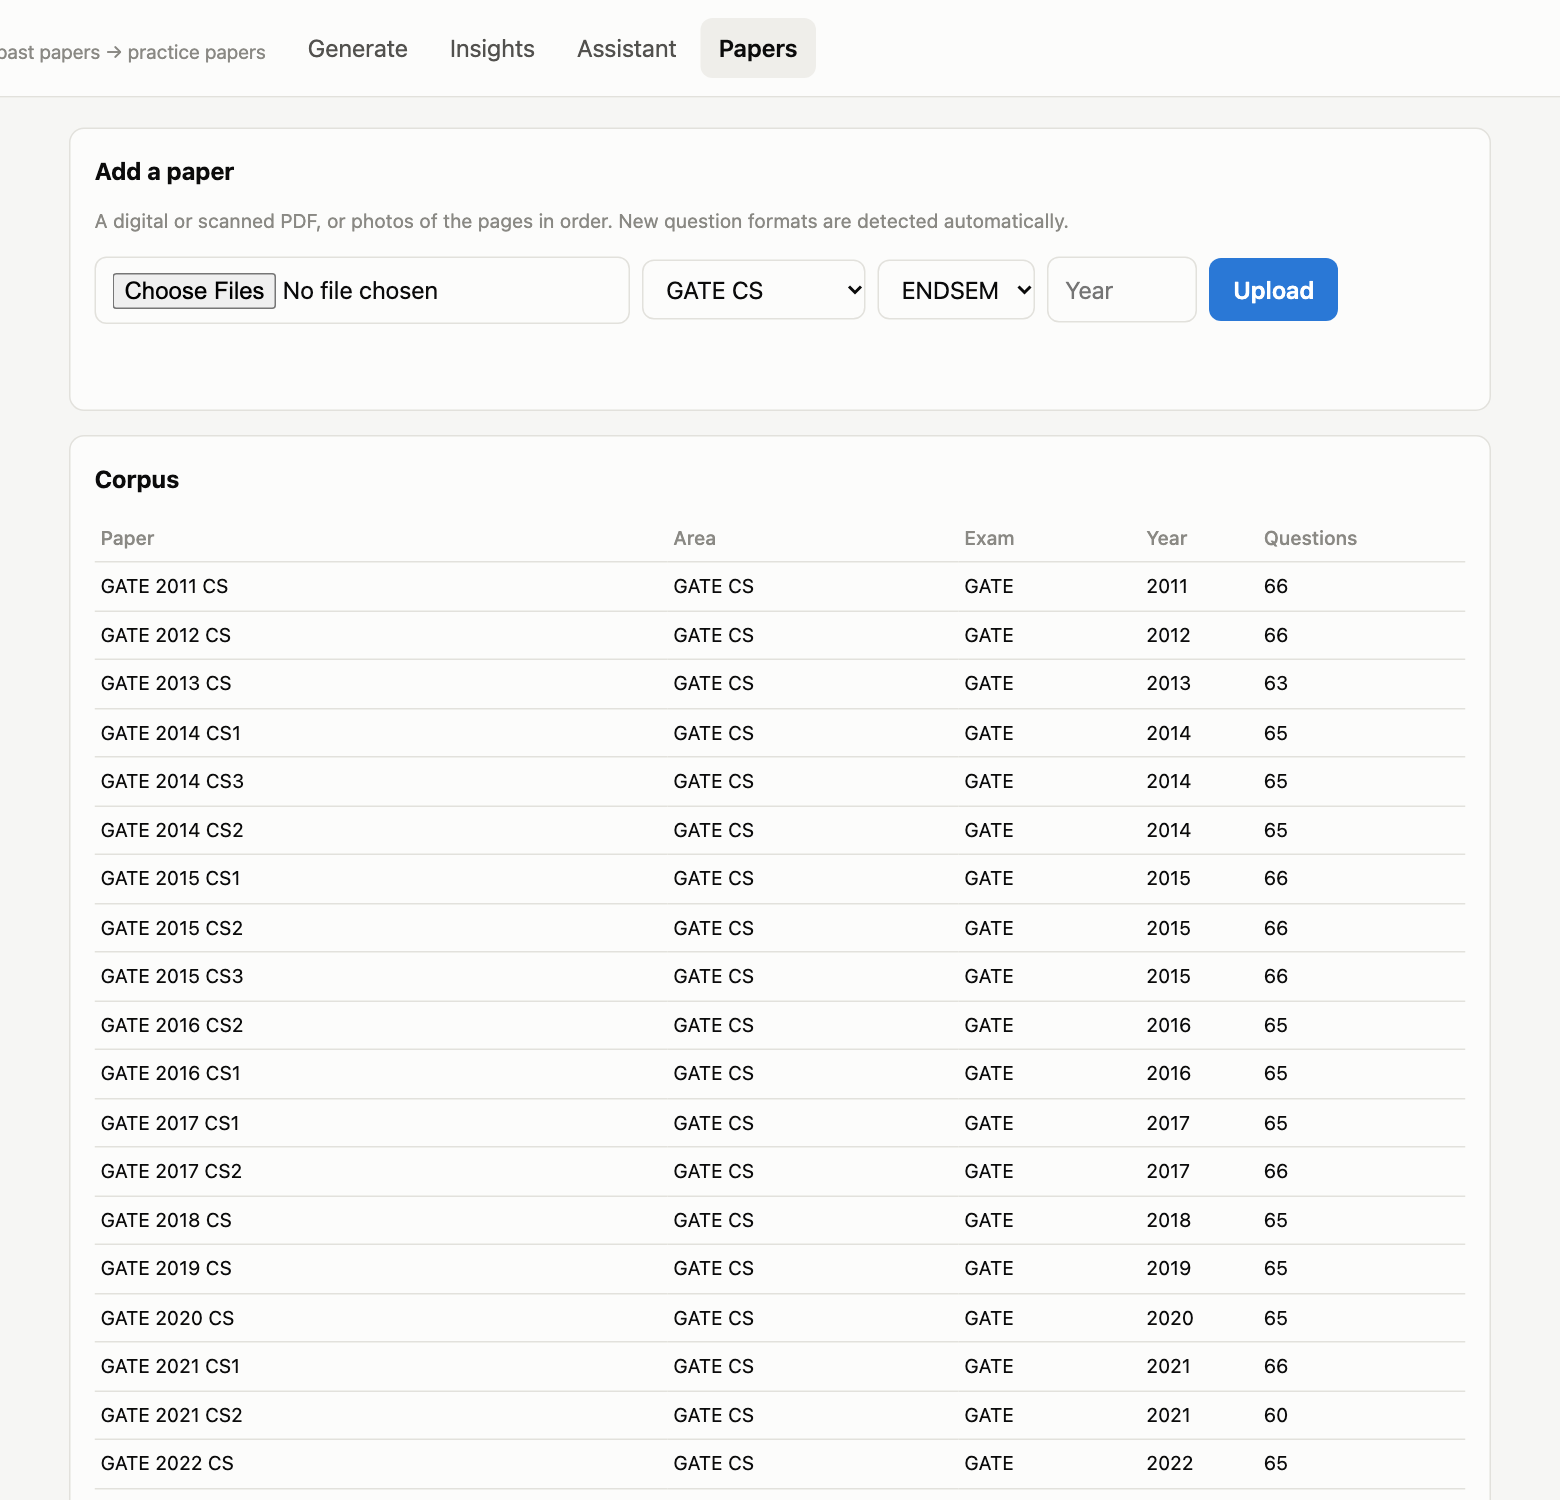
\includegraphics[width=0.9\textwidth]{figures/ui_papers.png}}{}
\caption{Papers tab: corpus listing and upload form for new scanned or digital papers}\end{figure}